\chapter{Экспериментальное исследование нелинейных эффектов в кристаллических микрорезонаторах} \label{chapt3}

\section{Изготовление кристаллических микрорезонаторов методом алмазного точения}

В литературе были продемонстрированы следующие способы изготовления микрорезонаторов:

\begin{itemize}
  \item Плавление в пламени водородной горелки для микросфер из плавленого кварца.
  \item Выжигание мощным лазером $CO_2$ вращающейся заготовки.
  \item Механическое точение резонаторов
  \item Различные литографические методы для изготовление интегральных микрорезонаторов
\end{itemize}

В данной работе для изговтовления всех микрорезонаторов из кристаллических материалов изучаося и использовался метод алмазного точения с последующей полировкой алмазными суспензиями.

Общий внешний микрорезонаторов представлен на рис. \ref{cavity_scheme_big}. Основные характеристики микрорезонатора - это диаметр, толщина цилиндра и радиус закругления боковой поверхности цилиндра, где сосредоточено поле мод шепчущей галереи.  Размеры варьируются в следующих пределах: диаметр от 100 мкм – 8 мм (в зависимости от необходимой ОСД $FSR= \frac{c}{2\pi Rn}$), толщина 0.1 мм – 2мм (в зависимости от толщины изначальной заготовки) и радиус закругления от 30 мкм до $R/2$ (где $R$ – радиус резонатора).

\begin{figure}[ht]
    \centering
  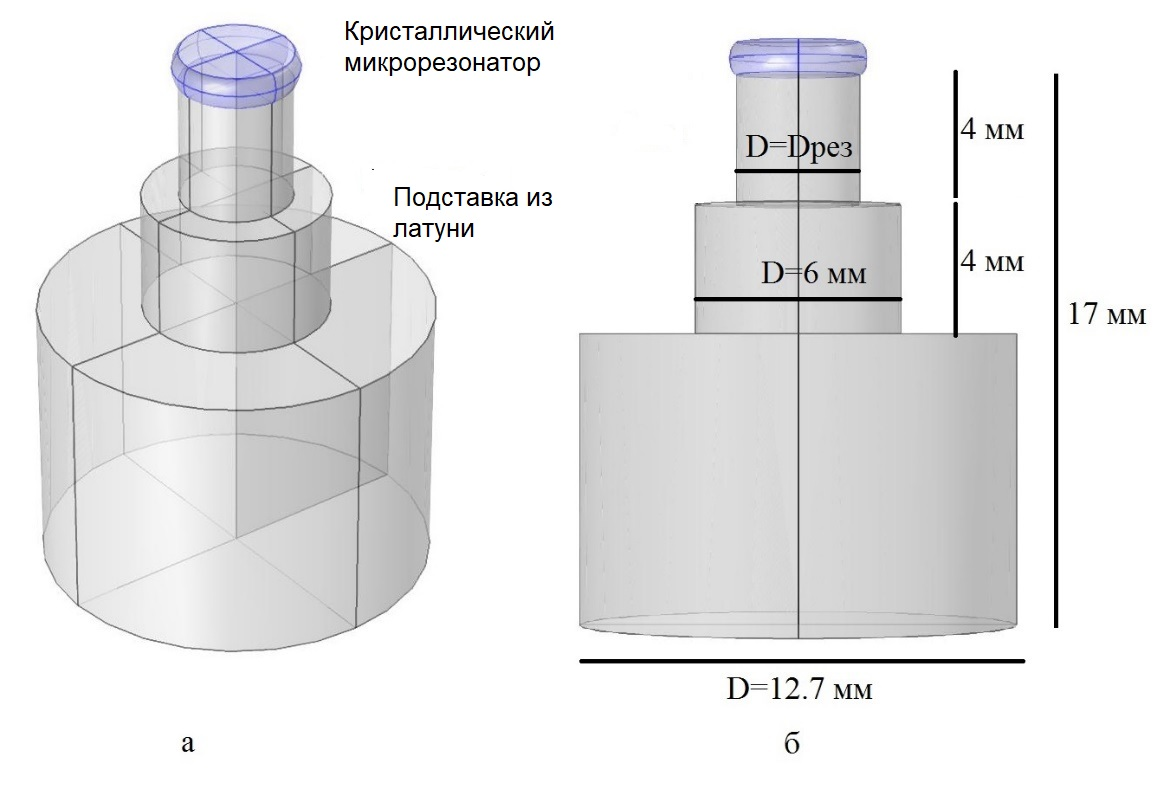
\includegraphics[width=0.5\linewidth]{cavity_scheme_big}
  \caption{Внешний вид кристаллического микрорезонатора и пьедестала: а – 3D вид, б – сечение XZ}
  \label{cavity_scheme_big}
\end{figure}

Для изготовления микрорезонатора с модами шепчущей галереи (ММШГ) использовались кристаллические пластины фторида магния ($MgF_2$), фторида кальция ($CaF_2$), фторида бария ($BaF_2$), фторида стронция ($SrF_2$), фторида лития ($LiF$), ниобата лития ($LiNbO_3$), танталата лития ($LiTaO_3$), кремния ($Si$), кристаллического кварца ($SiO_2$) и ряда других матералов.

Кристаллические микрорезонаторы из вышеуказанных материалов не могут быть изготовлены путем нагрева и обжига пламенем или мощным $СО_2$ лазером. Также пока не разработаны литографические способы их изготовления с необходимым качеством поверхности. Поэтому используется механическая обработка заготовок кристаллов в два этапа: точение алмазным резцом на прецизионном станке и последующая полировка алмазными пленками и суспензиями.

Ниже приведена последовательность действий, необходимых для изготовления микрорезонатора:

\begin{itemize}
  \item Наклеивание цилиндрической заготовки кристалла на латунную подставку с помощью УФ клея.
  \item Вытачивание цилиндра заданного диаметра алмазным резцом на станке алмазного точения (может выполняться изношенным резцом).
  \item Вытачивание на цилиндре микрорезонатора с заданной геометрией с помощью острого алмазного резца и программы для ЧПУ
  \item Очистка микрорезонатора с помощью салфетки, смоченной в изопропаноле или метаноле
  \item Проверка качества получившейся поверхности в микроскоп для обнаружения возможных шероховатостей, а также с помощью профилометра и методом проверки добротности
\end{itemize}

Хотя техника алмазного точения единственной точкой (SPDT, single point diamond turning) давно используется в большом количестве приложений, строгой теории для оптимального процесса точения нет. В процессе работы были экспериментально найдены оптимальные параметры для процесса точения.

Для алмазного точения использовался прецизионный станок с ЧПУ DAC ALM Lathe (рис. \ref{lathe}). Станок имеет прецизионный шпиндель на воздушных подшипниках и $2$ подвижные оси X,Y также на воздушных подшипниках. Точность подачи Х,Y специфицирована в $<10$ нм. Станок управляется с помощью программ, написанных на специально разработанном языке DSL. Станок оборудован высокоточным датчиком расстояния (LVDT), который измеряет расстояние по оси Y до момента касания заготовки. Также в комплекте к станку идет датчик высоты (профилометр), который измеряет изменение высоты с точностью до $0.1$ мкм. При двустороннем точении используется датчик, наносящий тонкие угловые отметки, позволяющие калибровать начало отсчета по оси C (угловое вращение шпинделя). Станок оборудован осциллирующим резцом, который синхронизируется с вращением шпинделя, и позволяет изготавливать асферические поверхности, а также выступы на фронтальной поверхности заготовки.

\begin{figure}[ht]
  \begin{minipage}[ht]{0.49\linewidth}\centering
    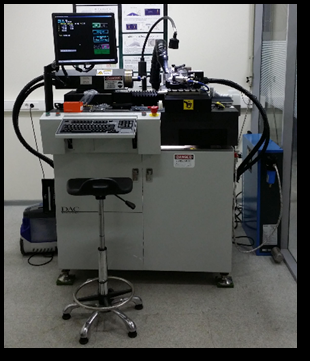
\includegraphics[width=1\linewidth]{lathe}
  \end{minipage}
  \hfill
  \begin{minipage}[ht]{0.49\linewidth}\centering
    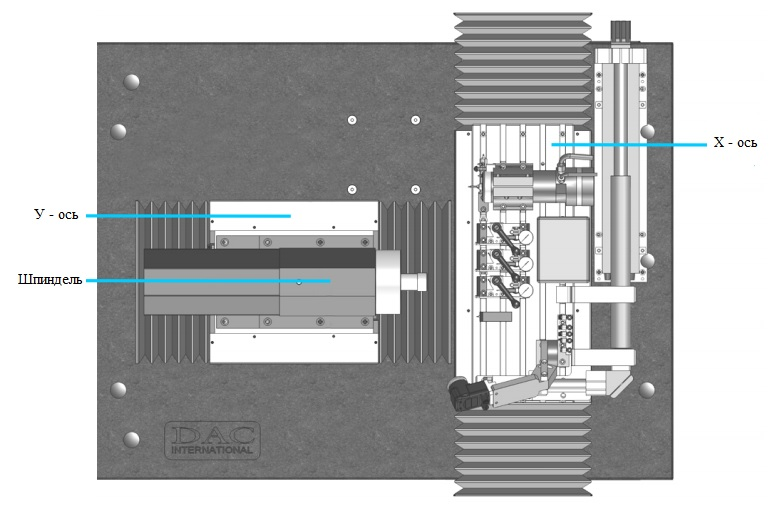
\includegraphics[width=1\linewidth]{lathe_top_view}
  \end{minipage}
  \caption{Прецизионный станок алмазного точения DAC ALM Lathe. Направление осей X,Y.}
  \label{lathe}
\end{figure}

Для точения использовались поликристаллические алмазные резцы производства KY Diamonds следующих типов (рис. \ref{diamond_tools}): 1) с радиусом кривизны 500 мкм, рабочей дугой окружности в 120 градусов, с 0 углом наклона рабочего края, конический задний угол резца 10 градусов; 2) с радиусом кривизны 100 мкм, рабочей дугой окружности в 60 градусов, с -25 углом наклона рабочего края, цилиндрический задний угол резца 8 градусов; 3) острый резец невыдержанным радиусом кривизны 4 мкм, 0 угол наклона рабочего края. Резцы располагались в держателе перпендикулярно (или под углом 80 градусов) оси вращения шпинделя со вставленным резонатором.

\begin{figure}[ht]
  \begin{minipage}[ht]{0.24\linewidth}\centering
    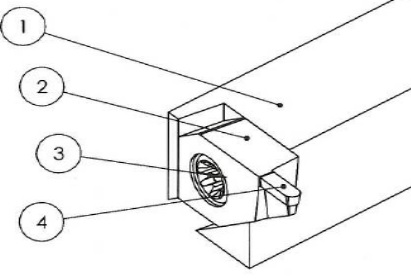
\includegraphics[width=1\linewidth]{tool1}
  \end{minipage}
  \hfill
  \begin{minipage}[ht]{0.24\linewidth}\centering
    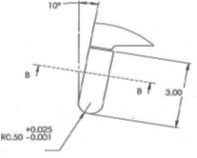
\includegraphics[width=1\linewidth]{tool2}
  \end{minipage}
  \hfill
  \begin{minipage}[ht]{0.24\linewidth}\centering
    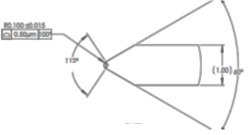
\includegraphics[width=1\linewidth]{tool3}
  \end{minipage}
  \hfill
  \begin{minipage}[ht]{0.24\linewidth}\centering
    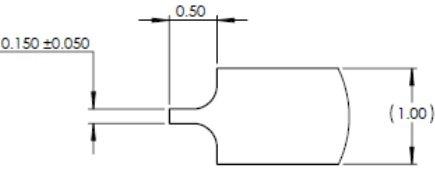
\includegraphics[width=1\linewidth]{tool4}
  \end{minipage}
  \caption{Чертежи используемых резцов.}
  \label{diamond_tools}
\end{figure}

Калибровка резцов проводилась по следующей методике:

\begin{itemize}
    \item В цангу вставляется заготовка (пластиковый цилиндр) диаметром 12.7 мм. Шпиндель подводится к калибруемому резцу. Выставляется на глаз отступ по оси Y до момента появления стружки (касания алмазного резца).
    \item Запускается программа, которая датчиком измеряет расстояние между фронтальной рабочей поверхностью до и после снятия слоя заданной толщины (например, 50 мкм). Точно зная это расстояние, окончательно калибруется зазор между датчиком расстояния LVDT и рабочей точкой резца.
    \item Запускается программа, наносящая штрих глубиной 1 мкм от края заготовки до ее центра (без вращения шпинделя). В оптический микроскоп (увеличение 40x) измеряется расстояние от центра заготовки до штриха (рис. \ref{tool_calibration}). Для правильной калибровки рабочая кромка резца изначально должна быть немного ниже центра. Используя датчик высоты, подстраивается высота калибруемого резца. Процедура повторяется до тех пор, пока штрих не будет проходить строго через центр заготовки.
    \item Проводится автоматическая калибровка расстояния по оси Х от рабочей точки алмазного резца до центра заготовки путем вытачивания трех концентрических окружностей: две при вращении шпинделя по часовой стрелке с одной стороны от центра, третья при вращении шпинделя в обратную сторону с другой стороны от центра. Далее измеряется получившееся расстояние между этими окружностями (с помощью датчика LVDT) и корректируется величина отступа между рабочей точкой резца и центром заготовки по оси X.
    \item В конце проводится калибровка расстояния по оси X до рабочей точки резца при точении цилиндра. Важно отметить, что точение фронтальной поверхности заготовки (перпендикулярно оси вращения шпинделя) и точение боковой поверхности цилиндра (параллельно оси вращения) осуществляется разными точками. Калибровка проводится путем вытачивания цилиндра заданного диаметра с последующим измерением получившегося диаметра с помощью микрометра. При необходимости расстояние по оси Х корректируется, и калибровка повторяется. Стоит подчеркнуть, что эта калибровка наименее точная из всех, т.к. погрешность микрометра при измерении диаметра цилиндра из мягкого пластика может составлять 3-5 мкм.
\end{itemize}


\begin{figure}[ht]
    \centering
  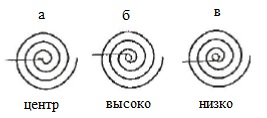
\includegraphics[width=0.5\linewidth]{tool_calibration}
  \caption{Результат калибровки высоты резца (правильная калибровка, резец высоко, резец низко).}
  \label{tool_calibration}
\end{figure}

Калибровка резцов осуществляется после каждой смены алмаза или при значительных дефектах обрабатываемых поверхностей.
Перед точением на станке из большой пластины материала резонатора вырезаются заготовки прямоугольной формы нужного малого размера. Для этого используется пила с алмазным диском, охлаждение производится водой.
Далее кристаллические заготовки наклеиваются на держатель (пьедестал) из пластика диаметром 12,7 мм, который соответствуют диаметру цанги на шпинделе станка. В работе использовались оптические клеи от производителя Norland Products (марки NOA 60, 61, 63, 65, 68), которые отвердевают при облучении УФ лампой. Клеи отличаются вязкостью в жидком виде, модулем упругости и твердостью в затвердевшем виде, оптическим показателем преломления и областью прозрачности. Все они не являются токопроводящими. Наилучший результат был достигнут с марками NOA 61, 65. Время облучения УФ лампой на длине 365 нм и мощностью 27 Вт/см$^2$ составляло 10 мин. Также использовались эпоксидная смола и этилцианакрилат, которые также давали хороший результат, но не позволяли долго центровать кристаллическую заготовку. Минимальный диаметр микрорезонатора, при котором не происходило отклеивание при точении, составил 700 мкм.
УФ клеи удобны для фиксации элементов ММШГ в крепежной сборке, т.к. позволяют юстироваться необходимое время и при отвердевании под УФ лампой не меняют свои размеры. После точения микрорезонаторы переклеивались на пьедестал меньшего диаметра или в крепежную сборку негабаритного макета. Все клеи размягчались и позволяли отклеить микрорезонатор при нагреве до 300-400 С. Также были испытаны двухкомпонентные клеи AremCo, который отвердевают за 24 часа при температуре 94 С, и выдерживают температуру нагревания до 400 С. Такой клей может использоваться при отжиге резонаторов.

Для центровки кристаллической заготовки в пластиковом пьедестале вырезалось отверстие глубиной 0.5 мм и диаметром, позволяющим разместить в нем заготовку. В отверстие заливался клей, помещалась заготовка и облучалась УФ лампой. Проверка центровки и перпендикулярности плоскости кристалла и оси вращения шпинделя проводилась визуально с помощью микроскопической трубы, подвешенной над шпинделем станка.

Были написаны программы на языке DAC DSL для вытачивания из цилиндрических кристаллических заготовок микрорезонаторов ММШГ со следующими профилями боковой поверхности: угловая, сферическая, прямоугольный выступ (рис. \ref{cavity_fab,cavity_small}). Параметры геометрии микрорезонатора настраиваются в широком диапазоне, ограниченном в основном геометрией самого алмазного резца.


\begin{figure}[ht]
  \begin{minipage}[ht]{0.49\linewidth}\centering
    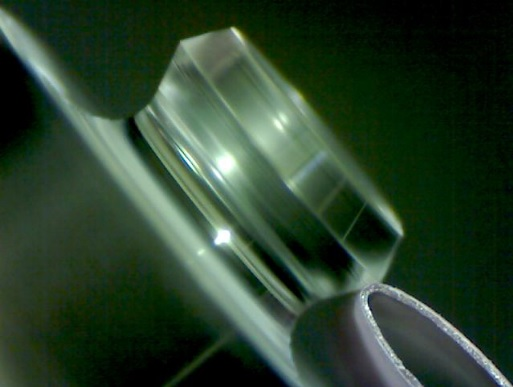
\includegraphics[width=1\linewidth]{cavity_fab_pad}
  \end{minipage}
  \hfill
  \begin{minipage}[ht]{0.49\linewidth}\centering
    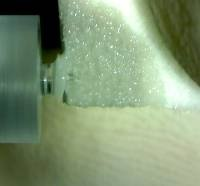
\includegraphics[width=1\linewidth]{cavity_fab_polishing}
  \end{minipage}
  \caption{Процесс ручной полировки алмазной шкуркой (слева) и алмазной суспензией (справа). Чистка резонатора проводилась на том же устройстве с использованием метилового спирта и салфеток Kimwipes.}
  \label{cavity_fab}
\end{figure}

\begin{figure}[ht]
\centering
  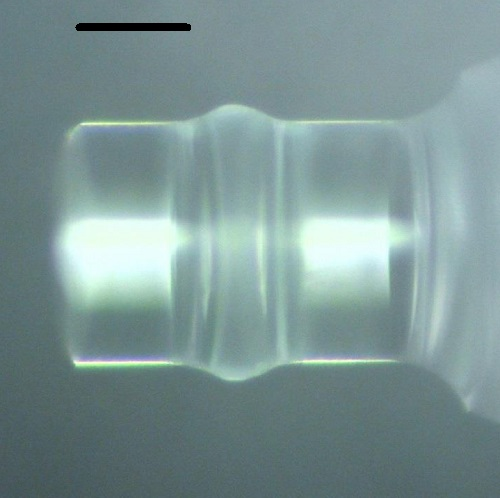
\includegraphics[width=0.5\linewidth]{cavity_fab_small}
  \caption{Микрорезонатор ММШГ ($MgF_2$) диаметром 250 мкм и радиусом кривизны боковой поверхности 50 мкм, выточенный с помощью программы DAC DSL.}
  \label{cavity_small}
\end{figure}

Алгоритм работы программы следующий:
\begin{itemize}
  \item Задаются начальные параметры (см рис. \ref{cavity_scheme})
  \begin{enumerate}
    \item диаметр заготовки (\texttt{blank\_diameter}),
    \item конечный внешний диаметр микрорезонатора (\texttt{diameter}),
    \item отступ от фронтальной (левой по рис. 32) поверхности (\texttt{front\_margin}), чтобы избежать возможных сколов у края
    \item хорда (\texttt{chord}), на которой располагается боковой выступ с радиусом кривизны (\texttt{curvature\_radius})
    \item высота (толщина) микрорезонатора ММШГ (\texttt{blank\_thickness})
    \item обороты шпинделя (\texttt{rpm})
    \item скорость движения резца при точении цилиндра (\texttt{cylinder\_fr}) и финального прохода с кривизной боковой поверхности (\texttt{fr})
    \item глубина захода резки при точении цилиндра (\texttt{cylinder\_step}) и финального прохода с кривизной боковой поверхности (\texttt{step\_amount\_to\_remove}).
  \end{enumerate}
  \item Грубым резцом стачивается цилиндр до нужного диаметра (направление движение резца параллельно оси вращения шпинделя) путем стачивания слоев высотой \texttt{cylinder\_step} со скоростью \texttt{cylinder\_fr}
  \item Финальным чистовым резцом (с радиусом кривизны алмаза, выдержанным с точностью 25 нм) последовательно стачиваются слои высотой \texttt{step\_amount\_to\_remove} с выступом сферической формы, передним отступом (\texttt{front\_margin}) и кривизной (\texttt{curvature\_radius}). Используется скорость движения резца \texttt{fr}.
\end{itemize}

\begin{figure}[ht]
\centering
  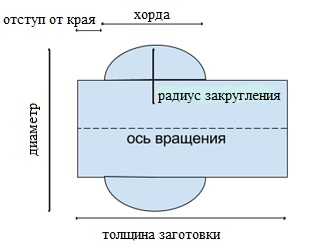
\includegraphics[width=0.5\linewidth]{cavity_scheme}
  \caption{Рисунок микрорезонатора ММШГ с параметрами для программы DAC DSL алмазного точения.}
  \label{cavity_scheme}
\end{figure}

Основными параметрами, влияющими на качество изготавливаемых микрорезонаторов ММШГ, являются скорость вращения шпинделя (rpm), линейная скорость точения (угловая скорость шпинделя умноженная на радиус резонатора), скорость движения резца (feed rate) и глубина захода (depth of cut). Опытным путем были определены следующие оптимальные параметры для точения кристаллов $MgF_2, CaF_2, BaF_2, LiNbO_3, LiTaO_3$:

\begin{itemize}
    \item rpm=400-1500;
    \item \texttt{feed\_rate}=2-3 мкм/оборот для предварительной обработки и <1-2 мкм/оборот для финального прохода;
    \item \texttt{depth\_of\_cut}=2-5 мкм для грубой обработки и 0.05-0.5 мкм для финального прохода.
\end{itemize}

Важнейшим фактором является охлаждение во время точения. Для этого на резец и резонатор распыляется охлаждающая жидкость, которая сразу же отсасывается в воздухозаборник вместе со срезанными стружками. В качестве охлаждения использовался изопропиловый спирт или Exxsol D100 – деароматизированная углеводородная жидкость. Жидкость не должна попадать внутрь шпинделя или линейных подач X,Y, а также должна быстро улетучиваться и не оставлять следов на кристалле. Без использования жидкости точение возможно, но с минимальной глубиной и скоростью подачи, при этом алмаз изнашивается значительно быстрее, а качество поверхности выточенного резонатора получается хуже.

После точения проводилась очистка микрорезонатора от кристаллической стружки с помощью полимерных салфеток, смоченных в метаноле. Сразу из-под резца получается добротность $10^5 -- 10^6$. Дальнейшее увеличение добротности достигается последовательной ручной полировкой с помощью и алмазных суспензий с уменьшающимся размером зерна (2.5 - 1 - 0.5 - 0.25 - 0.1 – 0.03 мкм) по 10-15 мин каждой. Использовались алмазные суспензии Microdiamant OPW-20, вязкость 325 cP, pH = 8.0, концентрация алмазных зерен 15 карат/литр. Суспензии наносились на тканный текстиль AlliedHighTech. Преимуществом использования суспензий, нанесенных на мягкую текстильную подложку является возможность более плотного контакта с тороидальной поверхностью по сравнению с алмазными шкурками на полимерной пленке.

Важнейшим элементом процедуры является очистка резонатора после полировки каждой шкуркой. Очистка проводилась теми же средствами, что и первичная очистка после точения, и длилась по 5 мин. При длительном нахождении микрорезонатора ММШГ в пыльном месте, может потребоваться повторная очистка для достижения максимальной добротности.

На рис. \ref{cavity_polished} приведены фотографии поверхностей микрорезонатора ММШГ сразу после точения изношенным резцом, фрагмент со сколом и после полировки алмазными суспензиями. Видно значительное улучшение качества поверхности.

\begin{figure}[ht]
  \begin{minipage}[ht]{0.32\linewidth}\centering
    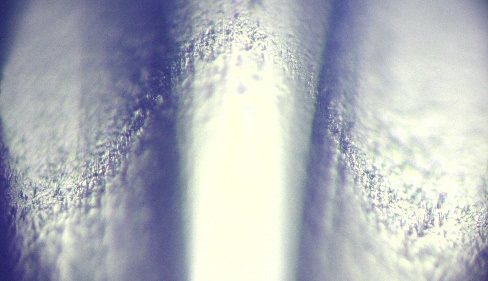
\includegraphics[width=1\linewidth]{cavity_unpolished}
  \end{minipage}
  \hfill
  \begin{minipage}[ht]{0.32\linewidth}\centering
    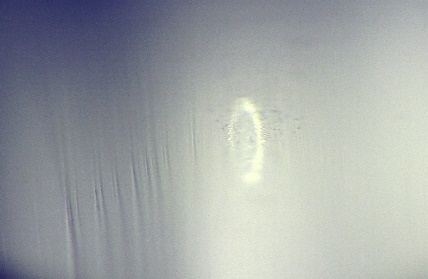
\includegraphics[width=1\linewidth]{cavity_polished_bad}
  \end{minipage}
  \hfill
  \begin{minipage}[ht]{0.32\linewidth}\centering
    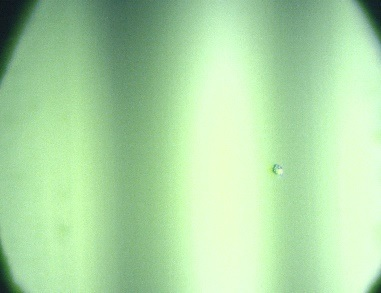
\includegraphics[width=1\linewidth]{cavity_polished_good}
  \end{minipage}
  \caption{Фрагмент поверхности резонатора с радиусом кривизны боковой поверхности 50 мкм (ширина выступа около 70 мкм). Слева сразу после точения изношенным резцом. Посередине фрагмент со сколом размером 20 на 50 мкм. Справа - после полировки алмазными суспензиями.}
  \label{cavity_polished}
\end{figure}

При увеличении глубины резки (depth of cut) до 6 мкм и более возможен хрупкий режим точения со сколами кристалла и повышенным износом резца. После очистки микрорезонатора проводится проверка качества получившейся поверхности в микроскоп для обнаружения возможных шероховатостей.

Так как обычный оптический микроскоп имеет дифракционный предел, дефекты малого размера в нем не видны, и на большом увеличении глубина резкости минимальна, видна очень малая область тороидальной боковой поверхности (не более 10-20 мкм), то контроль качества осуществлялся последовательным измерением добротности мод после полировки новыми алмазными суспензиями.

Дополнительно может быть произведен контроль качества боковой поверхности с помощью оптического профилометра Zygo NewView 7300. Результат измерения приведен на рис. \ref{cavity_profilometer}, измерены шероховатости размером 0.25 мкм.

\begin{figure}[ht]
\centering
  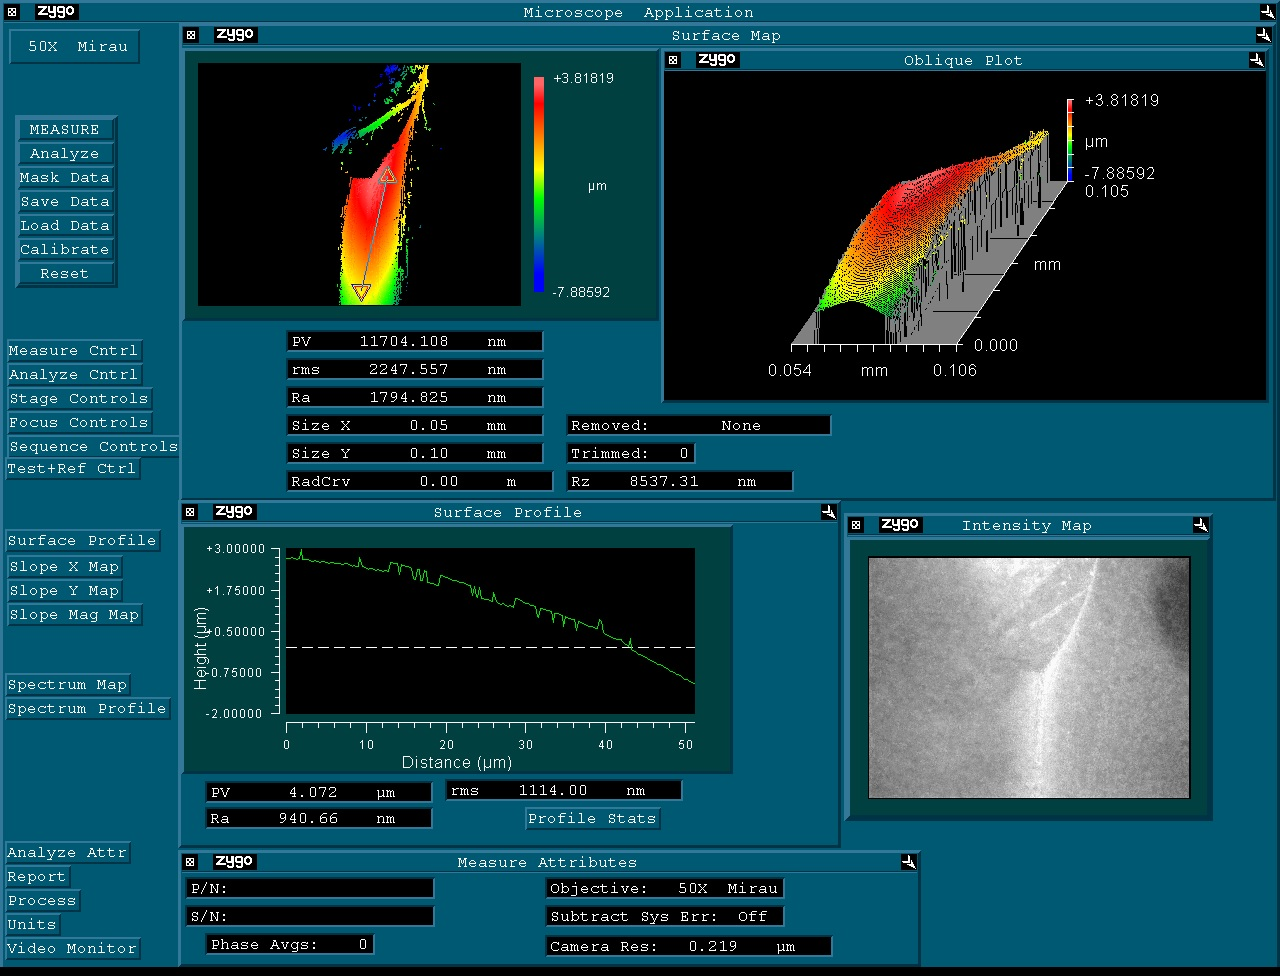
\includegraphics[width=0.5\linewidth]{cavity_profilometer}
  \caption{Измерение качества боковой поверхности с помощью оптического профилометра}
  \label{cavity_profilometer}
\end{figure}

Достаточным условием для оценки качества поверхности является проверка добротности после полировки. К сожалению, при таком способе оценки качества поверхности можно упустить технические ошибки, возникающие при полировке, т.к. в данном случае о качестве можно судить только по косвенному признаку – добротности. Измерение добротности производилась следующими методами: калибровка частоты дается боковыми линиями фазовой модуляции сканирующего лазера, зная частоту модуляции, можно аппроксимировать лоренцевскую форму резонанса МШГ. Для измерения ширины линии резонанса меньше 500 кГц лучше использовать метод звона, при котором либо быстро выключается, либо быстро перестраивается по частоте лазер накачки и проводится прямое измерение времени звона оптического резонатора по затухающему сигналу фотодетектора. Для измерения сверхвысоких добротностей необходимо использовать мощность лазера меньше 1 мВт, чтобы избежать нелинейных уширений.

В таблице \ref{table_turning_params} представлены параметры точения, при которых получались наилучшие результаты для различных материалов. 

\begin{table} [htbp]% Пример записи таблицы с номером, но без отображаемого наименования
	\centering
	\parbox{17cm}{% чтобы лучше смотрелось, подбирается самостоятельно
        %\captionsetup{format=tablenocaption}% должен стоять до самого caption
        \caption{Параметры алмазного точения резонаторов из различных кристаллических материалов}%
        \label{table_turning_params}%
    	\begin{tabular}{||c|c|c|c|c||}
\hline
\multicolumn{1}{|p{2cm}|}{\centering Материал} & \multicolumn{1}{|p{2cm}|}{\centering Скорость вращения шпинделя \\ обороты в мин} & \multicolumn{1}{|p{2cm}|}{\centering Скорость движения резца \\ мкм/оборот} & \multicolumn{1}{|p{2cm}|}{\centering Глубина захода резки \\ мкм} & \multicolumn{1}{|p{2cm}|}{\centering Охлаждающая \\ жидкость}\\
%Материал & Скорость вращения шпинделя, обороты в мин & Скорость движения резца, мкм/оборот & Глубина захода резки, мкм & Охлаждающая жидкость\\
\hline
$MgF_2$ & 400-1500 & 0.25-1 & 0.5-1 & да/нет \\
\hline
$BaF_2$ & 1000-2500 & 1-2.5 & 0.5-2 & нет \\
\hline
$CaF_2$ & 700-2500 & 1-2 & 1 & да/нет \\
\hline
$LiNbO_3$ & 900-1500 & 1-2.5 & 1-4 & нет \\
\hline
$LiTaO_3$ & 900 & 1-2 & 1-2 & нет \\
\hline
$Si$ & 500 & 1 & 0.5-1 & да \\
\hline
$TGG$ & 700 & 1 & 0.5-1 & нет \\
\hline
\end{tabular}

	}
\end{table}

\subsection{Практические замечания по изготовлению кристаллических микрорезонаторов}

Предобработка - раскол кристаллических пластин заготовок, при этом возможно образование напряжений внутри кусочков кристаллов. Мягкие материалы $BaF_2, CaF_2$ раскалываются на неконтролируемые куски при любой толщине заготовки. Распил алмазной пилой позволяет этого избежать. Однако для заготовок толщиной 100-200 мкм возможны внутренние трещины из-за неровности наклейки на подставку для распила. Необходимо использовать тонкие диски пилы с алмазным напылением. Выпиливание цилиндрических заготовок трубчатым сверлом малоэффективно, т.к. большая часть материала уходит в стружку и из-за больших биений сверла вероятно появление больших сколов.

Дизайн подставки \ref{cavity_scheme_big} диктуется размером цанги станка и удобством крепления в экспериментальных установках. Материал подставки латунь выбран из-за достаточно высокой теплопроводности для улучшения активной термостабилизации. Все кристаллические материалы для генерации оптических гребенок имели z-cut, т.ч. оптическая ось z совпадала с осью цилиндра.

Отжиг кристаллов для устранения внутренних дефектов проводился, но без прямого измерения улучшения добротности до и после, т.к. клей не позволяет нагревать до 700-800С наклееный на подставку резонатор, а в случае переклейки резонатора вероятность загрязнения велика и будет требоваться новая переполировка. При попытке отжига наклеенного резонатора из $BaF_2$ при 400С в кристалле возникло большое количество внутренних трещин.

Алмазное точение SPDT возможно в широком диапазоне параметров при использовании нового неизношенного резца. Качество поверхности фторида магния при этом высокое, т.ч. добротность резонатора может достигать $10^6$ (пример выступа резонатора с такой добротностью дан на рис. \ref{protrusion_unpolished}), что соответствует типичным значениям добротности в интегральных оптических резонаторах.

\begin{figure}[ht]
\centering
  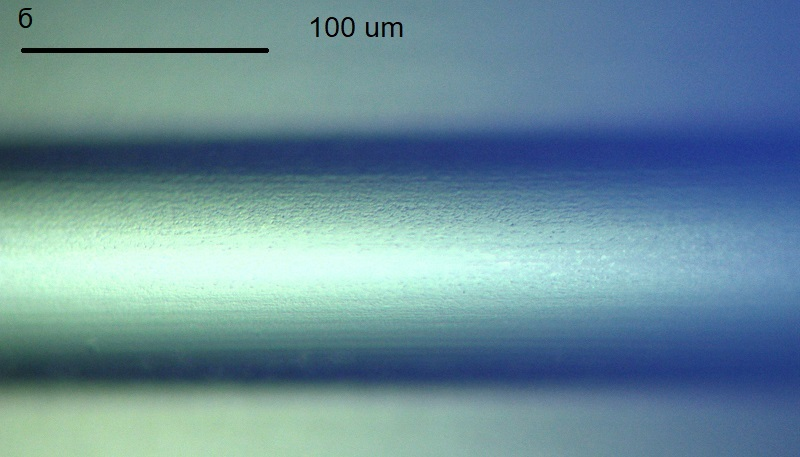
\includegraphics[width=0.5\linewidth]{protrusion_unpolished}
  \caption{Фотография поверхности резонатора из $MgF_2$ сразу после точения, в котором достигается добротность $10^6$ на 1550 нм.}
  \label{protrusion_unpolished}
\end{figure}

Основной недостаток метода алмазного точения - быстрый износ алмазного резца. На практике износ резца наступает за 100 м точения, что соответствует изготовлению 3 резонаторов. Далее качество получаемой поверхности заметно ухудшается и никакими более щадящими параметрами точения улучшить его нельзя. Изношенным резцом возможно точение твердых материалов $MgF_2$, но более мягкие $BaF_2, LiF$ могут давать сколы размерами в несколько сот микрон, недоступными для устранения полировкой \ref{cavity_damage}. Наиболее практично использовать для изготовления цилиндров заданного диаметра изношенный резец, а далее снимать финальный слой толщиной 10 мкм с помощью чистового неизношенного резца. Важно при этом регулярно проводить перекалибровку относительного положения изношенного и чистового резцов, т.к. сколы края алмаза могут достигать 10 мкм \ref{tool_damage}.

\begin{figure}[ht]
  \begin{minipage}[ht]{0.49\linewidth}\centering
    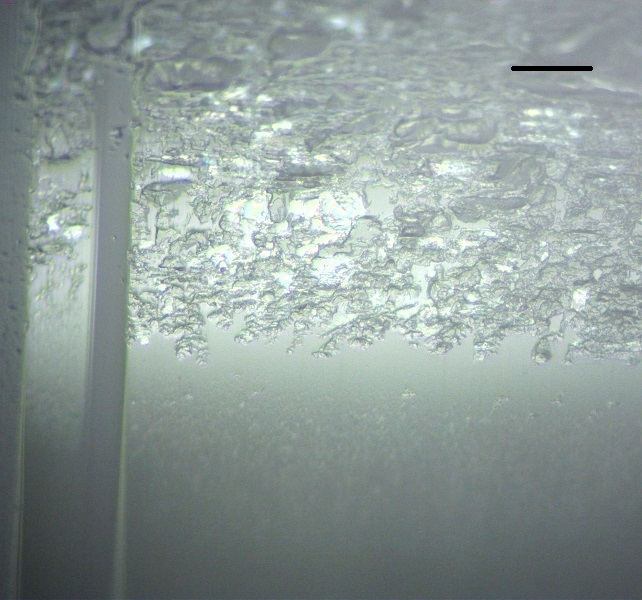
\includegraphics[width=1\linewidth]{cavity_damage}
  \end{minipage}
  \hfill
  \begin{minipage}[ht]{0.49\linewidth}\centering
    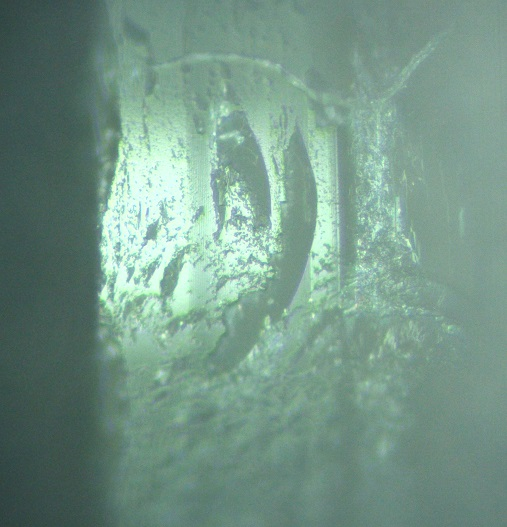
\includegraphics[width=1\linewidth]{cavity_damage_baf2}
  \end{minipage}
  \caption{Слева фрагмент поверхности резонатора из $MgF_2$ после точения при неоптимальных параметрах, видны секторы хорошего и плохого качества поверхности, соответствующие точению различных кристаллических срезов, такие дефекты можно убрать полировкой без сохранения геометрии резонатора. Справа фрагмент поверхности резонатора из $BaF_2$ после точения изношенным резцом, видны глубокие сколы, которые нельзя убрать полировкой.}
  \label{cavity_damage}
\end{figure}

\begin{figure}[ht]
\centering
  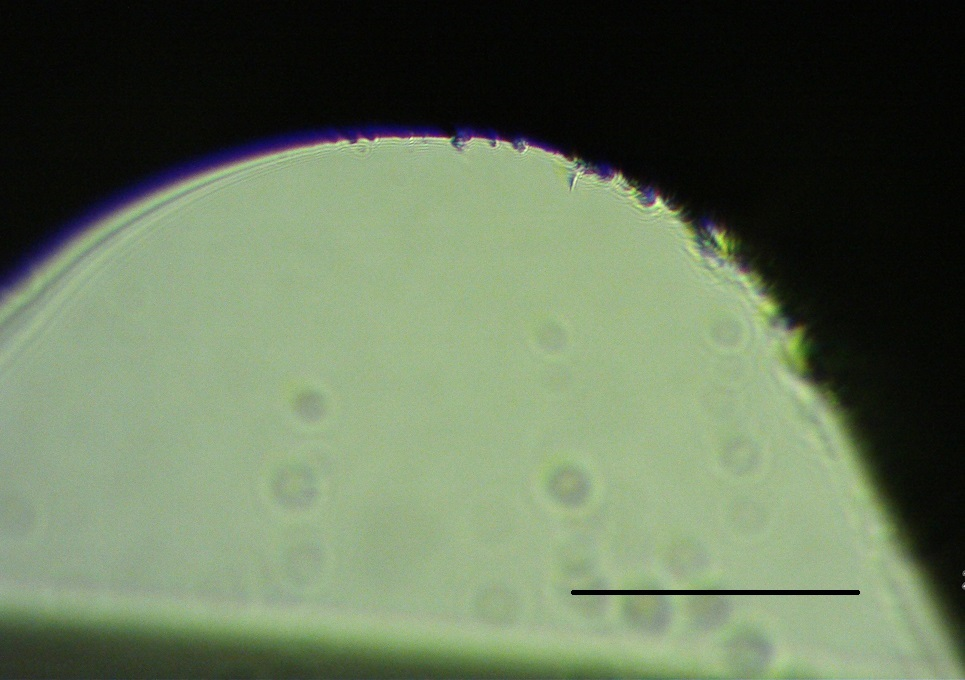
\includegraphics[width=0.5\linewidth]{tool_damage}
  \caption{Рабочий край изношенного алмазного резца с радиусом кривизны 500 мкм, видны сколы по краю характерным размером 10 мкм. При дальнейшем использовании резца возможно образование скола алмаза по прямой линии, таким резцом можно грубо вытачивать цилиндры заданного диаметра.}
  \label{tool_damage}
\end{figure}

В литературе по точению основными методами борьбы с износом являются более щадящие параметры точения (уменьшение глубины резки и действующей силы, пропорциональной скорости вращения) и использовании охлаждающей жидкости. Важно понимать, что при использовании охлаждающей жидкости меняется режим точения и следует заново подбирать оптимальные параметры. Уменьшение же глубины резки приводит к пропорциональному росту времени точения. Охлаждающая жидкость при изготовлении большинства резонаторов из $MgF_2$ не применялась, т.к. нет удобной системы вентиляции, и ее расход велик, т.ч. бака может не хватать на типичное точение в 6-10 часов, также заводская жидкость содержала маслянистые фракции, которые могут повредить шпиндель на воздушных подшипниках.

Полировка при хорошей центровке микрорезонатора возможна не только последовательным уменьшением зерна суспензии, но и при грубой полировке зерном 2.5-4 мкм для удалений сколов с характерными размерами 5-15 мкм, далее зерном 0.5 мкм и сразу 0.1 мкм для финальной полировки. Стандартное правило - удаление материала в 3-4 кратном размере диаметра зерна. Таким способом повторяемо достигается добротность $5*10^8$ на длине волны $1550 нм$ в кристаллах $MgF_2$ из заготовки VUV качества материала.

Изготовление прямоугольных микровыступов даже новыми острыми резцами не удалось для диаметров резонатора больше 4 мкм для $MgF_2$ и получилось для диаметров около 1 мм \ref{protrsuion_rect}. Этот резонатор далее детально не изучался.

\begin{figure}[ht]
\centering
  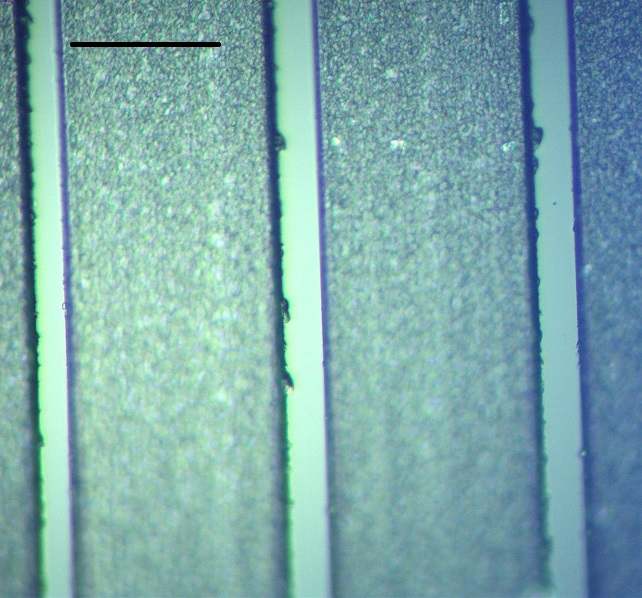
\includegraphics[width=0.5\linewidth]{protrsuion_rect}
  \caption{Фрагмент поверхности резонатора с прямоугольными выступами размером 5 на 15, 20, 25 мкм для контроля ДГС резонатора. Показано качество поверхности до полировки, видны сколы по 5 мкм на выступе из-за износа острого резца.}
  \label{protrsuion_rect}
\end{figure}

\section{Экспериментальное наблюдение оптических частотных гребенок и солитонов в резонаторах из $MgF_2$}


\subsection{Экспериментальное установка и результаты генерации солитонов}

Схема

Описание моделей оборудования

Примеры шумных гребенок (самая широкая и 12 ГГц)ю

Солитон 8 ГГц, 26 ГГц, 12 ГГц, состояния с большим количеством мод кроссингов, но узким битноутом

\subsection{Методы контроля и стабилизации частоты и отстройки лазера накачки}
метод VNA, обзор работы Карпова, возможно картинка RIGOL

более удобный метод PDH, мину - нет возможности менять отстройку

\subsection{Метод стабилизации частоты повторения солитонов с помощью амплитудной модуляции лазера накачки}
амплитудная модуляция на кратных фср частотах приводит к узкой области захватывания частоты повторения солитонов

\subsection{Метод достижения односолитонного режима с помощью модуляции лазера накачки}

Перевод от хаоса к порядку экспериментальной части.

\section{Экспериментальное наблюдение двойных оптических частотных гребенок в резонаторах из $MgF_2$}

\subsection{Генерация двух солитонных оптических гребенок в двух резонаторах на одном цилиндре}

In this Letter, we present a compact optical dual-comb source based on ultra-high Q-factor crystalline MgF$_2$ optical whispering gallery mode (WGM) microresonators pumped by continuous wave lasers which may be used for compact spectroscopy or LIDAR applications. Although crystalline microresonators were the first microresonator platform in which dissipative solitons were generated, which have been applied already to low noise microwave generation[Matkso] and for creating an RF to optical link [Optica], achieving dual comb spectroscopy is challenging due to the requirements on the repetition rates. Here it is shown that resonators with almost identical FSR can be fabricated on the same crystalline preform. This enables the FSR of the microresonators $\sim 12.1$~GHz with a difference of only $1.62$ MHz. The demonstrated dual comb source allows the downconversion of an optical soliton frequency combs spanning $30$~nm ($3.7$~THz) near $1554$~nm to a narrow span of $300$~MHz in the RF domain.

\section{Cavity design and fabrication}
For a simultaneous generation of several soliton frequency combs with almost identical repetition rate, we developed a structure consisting of several identically shaped magnesium fluoride microresonators cut on the same crystalline rod as shown in [Fig.\ref{ris:image1}]. The structure had $5$ equal protrusions with a curvature radius of $35$~µm and a diameter of $5.68$~mm corresponding to a FSR $\sim 12.1$~GHz. The distance between adjacent protrusions was $140$~µm. This stack of microresonators was manufactured by single-point diamond turning (SPDT) technique \cite{Tanabe:16}, using an ultra-precise computer-controlled lens lathe (DAC ALM).

\begin{figure}[ht]
\begin{minipage}[ht]{1\linewidth}
\center{\includegraphics[width=0.9\linewidth]{img/fig1}}
% * <erwan.lucas@epfl.ch> 2016-11-17T11:44:23.151Z:
%
% This figure needs a bigger text ! This is way too small
%
% ^.
\end{minipage}
\caption{ (a): View of the WGM cavities on a single crystalline rod with a major diameter of $5.68$~mm, minor diameter of $35$~µm, and distance between adjacent protrusions of $140$~µm. The inset shows $3$ unpolished cavities (\#2 -- \#4) after single point diamond turning where solitons were observed. (b-d): optical single soliton spectra generated from $3$ different cavities (\#2 -- \#4). The soliton Kerr frequency combs spans $30 - 65$~nm with a line spacing of $12.1$~GHz;}
\label{ris:image1}
\end{figure}

The quality factor after diamond cutting was approximately 10$^6$. The ultra-high intrinsic Q-factor exceeding $10^9$ was achieved by asymptotic polishing with diamond slurries \cite{Maleki:01}. To preserve the initial accuracy of the manufacturing, lint-free wipes with polishing diamond slurries were controllably applied with the same pressure to three chosen adjacent protrusions simultaneously (numbers $2 - 4$ in [Fig.\ref{ris:image1}(a)]). As a result of fine polishing, the difference between the FSR of several protrusions was below $10$~MHz indicating a difference of radii at the level of $0.5 - 1$~µm assuming excitation of similar mode types, sufficient for dual comb spectroscopy applications.
The loaded Q-factors of the three specially polished microresonators were ~10$^9$ after the smallest grain size polishing. The Q-factors of the other protrusions less affected by polishing procedure were $10^8$ and below.

\section{Experimental results}

\begin{figure}[ht]
\begin{minipage}[ht]{1\linewidth}
\center{\includegraphics[width=1\linewidth]{img/Setup}}
\end{minipage}
\caption{Experimental setup to generate the soliton dual comb RF beating from the protrusions \#2 and \#4. CW: continuous-wave narrow linewidth tunable fiber laser; EDFA: erbium-doped fiber amplifier; AFG: arbitrary function generator; FPC:  fiber polarization controller; FBG: fiber Bragg grating; PD: photodetector; ESA: electrical spectrum analyzer; OSA: optical spectrum analyzer; OSC: oscilloscope.}
\label{ris:image2}
\end{figure}

A schematic view of the experimental setup is shown in Fig.\ref{ris:image2}. Two continuous-wave tunable narrow linewidth fiber lasers ($\lambda \sim 1554$~nm) were amplified with erbium-doped fiber amplifiers and coupled into the WGM resonators via two tapered optical fibers \emph{[TJK cite PRA J. Hofer which first demonstrated this for crystals]}. Each tapered fiber approached a distinct resonating protrusion (\#2 and \#4) from opposite sides and excited solitons with different FSRs. An arbitrary function generator was used to control the soliton generation in both microresonators via frequency detuning of the lasers \cite{Kippenberg:14}. Fiber polarization controllers were added to optimize the coupling efficiency. A fiber Bragg grating  was employed to suppress the transmitted pump power in the out-coupled optical signals. The repetition rates of the soliton pulses were monitored with a fast photodiode (25 GHz bandwidth) and an electrical spectrum analyzer. An optical spectrum analyzer recorded the optical comb spectra from both microresonators. The piezo-voltage of the frequency swept lasers and the transmitted optical power for both protrusions, showing the characteristic step pattern, indicating the soliton formation, were monitored with an oscilloscope.

\begin{figure}[ht]
\begin{minipage}[ht]{1\linewidth}
	\center{\includegraphics[width=0.8\linewidth]{img/fig3}}
\end{minipage}
\caption{(a-b): Optical multisoliton spectra generated separately from cavities $\#2$ and $\#4$; (c): FSR beatnote spectrum of two simultaneous multisoliton states in two different cavities used for dual comb generation, FSR difference is $1.62$ MHz.}
\label{ris:image3}
\end{figure}

In our 5-cavity structure, Kerr soliton frequency combs were observed in three different neighboring microresonators [Fig.\ref{ris:image1}]. The width of the optical soliton spectra shown in [Fig.\ref{ris:image1}(b) -- Fig.\ref{ris:image1}(d)] covered 30 to 65~nm around $1554$~nm. The difference between laser pump wavelengths used to excite different resonators was $8.9-30$~pm. Two soliton trains having different repetition rates $\Delta \mbox{FSR} = \mbox{FSR}_1 - \mbox{FSR}_2 = 1.62$~MHz were simultaneously generated from two different protrusions of the crystalline rod (\#2 and \#4 in [Fig.\ref{ris:image1} (a)]) and then combined using a fiber splitter.

To generate the dual soliton comb, we used the laser tuning method first proposed in \cite{Kippenberg:14}. We applied the ramp voltage to both lasers and tuned into the soliton state simultaneously in both cavities. The ramp starting frequency of the lasers were adjusted by aligning the characteristic soliton steps in the transmission signals from both cavities.

Optical spectra of multisoliton combs in both resonators are presented in [Fig.~\ref{ris:image3}(a) -- Fig.~\ref{ris:image3}(b)], the narrowest comb in [Fig.~\ref{ris:image3}(b)] contains $350$ lines separated by $12.1$~GHz and spans $35$~nm around the center wavelength $\lambda = 1554$~nm. The FSR beat note spectrum of multisoliton state combs in both resonators is shown in [Fig.\ref{ris:image3}(c)], FSR difference between two resonators is $1.62$~MHz and the pump lasers frequency difference is $1.07$~GHz. The dual comb downconversion from the optical domain to the RF domain [Fig.\ref{ris:image4}] results in a $300$~MHz wide RF comb, centered at $1.07$~GHz, consisting of $160$ lines spaced by $1.62$~MHz, and having a spectral envelope resulting from the optical spectrum of the two multisoliton combs. The obtained multisoliton dual comb state was short-lived ($\sim 30$ seconds), although, independently, soliton states in each cavity existed for minutes without any additional stabilization techniques.

\begin{figure}[ht]
\begin{minipage}[ht]{1\linewidth}
\center{\includegraphics[width=0.8\linewidth]{img/fig4}}
% THE DBM AND FREQ. UNIT SHOULD BE IN PARENTHESIS
\end{minipage}
\caption{Radio-frequency spectrum resulting from heterodyning two multi-soliton Kerr frequency optical combs. The RF dual comb covers $300$~MHz around $1.07$~ GHz with ~$160$ lines separated by $1.62$~MHz.}
\label{ris:image4}
\end{figure}

The short lifetime of the dual comb state is due to the thermal resonance frequency shift, which makes the presented method challenging. The soliton excitation in one cavity was observed to lead to a thermally-induced resonance frequency shift in the other cavity, thus moving its effective detuning out of the soliton existence range. As a result, we consistently obtained a soliton comb in one cavity and a high noise or MI comb state in the other cavity.

Thermal frequency shifts in all 5 cavities were simulated using finite element method with Comsol Multiphysics software. The simulated cavity geometry coincides with the actual fabricated device: cylindrical MgF$_2$ rod is placed on a brass pedestal and cavities $\#2$ and $\#4$ are heated due to the circulating optical power. The characteristic power of 50 mW is assumed to be dissipated as heat. The material parameters were taken from the supplier site (Crystran). We simulated the temperature variation and thermal expansion in the system assuming the heat sources were turned on simultaneously. Then the frequency shifts were obtained using the simple relation
\begin{align}
\frac{\Delta f}{f}=-\beta\frac{\Delta T}{n}-\frac{u_r}{R},
\end{align}
where $n$ is refraction index, $\Delta T$ is temperature change, $\beta$ is thermal refraction coefficient, $u_r$ is radial displacement of the boundary caused by thermal expansion and $R$ is unperturbed radius. [Fig.\ref{ris:image5}] shows the resulting resonance frequency shifts in different cavities, the inset shows the result for thermal expansion in stationary regime. The mechanical part was found to give out more effect than the refractive one. The simulations demonstrated that pumping one of the resonators significantly shifts the resonance frequencies of all other resonators reaching a steady state in a $1$-s timescale. In our experiment, the typical thermal frequency shifts were between $30-50$~MHz, which is in good agreement with the numerical simulation results (the resonance shift between cavities 2 and 4 is~$50$ MHz at $1$~s). However, the simulations  indicate that the thermal influence can be significantly reduced, by fabricating cavity protrusions separated by approximately $2$~mm or by adding a heat sink at both the top and bottom of the crystalline cylinder. The shift was also shown to depend linearly on intracavity power. In this way, we anticipate that the issues posed by the thermo-optic effects may be mitigated by appropriate design and active thermal stabilization, such as via recently developed techniques that stabilize the soliton duration [cite Nat. Phys. and Vahala OL].

\begin{figure}[h]
\begin{minipage}[ht]{1\linewidth}
\center{\includegraphics[width=1\linewidth]{img/fig5}}
% THE SIMULATION INSET SHOULD HAVE BIGGER FONT AND PROPER UNITS (MM) AND THE COLOR SCALE UNITS INDICATED
\end{minipage}
\caption{Numerical modeling of the resonance frequency shift induced by thermorefraction and thermal expansion of the 5-cavity system. Inset -- displacement caused by heating (increased 50000 times for visualization) in stationary regime.}
\label{ris:image5}
\end{figure}


\section{Conclusion}
In this Letter we present a precise fabrication technique of crystalline whispering gallery microresonators that allowed us to achieve FSR difference down to $\sim 1.6$~MHz. We fabricated a novel structure with several identical microresonators on a single MgF$_2$ crystalline rod with a diameter difference of only $\sim 500$~nm and demonstrated a soliton dual comb source from such structure, enabling the down conversion of $3.7$~THz of optical span centered at $\lambda \sim 1554$~nm to a $300$~MHz RF comb centered at $1.07$~GHz. Full thermomechanical modelling of the system was performed and mitigation methods for thermal effects influence were discussed. Such compact dual comb sources open promising applications perspectives in spectroscopy and laser ranging.




\section{Экспериментальное наблюдение вынужденного рассеяний Рамана и Бриллюэна в резонаторах из $MgF_2$}
